\chapter{Fluoride Salt Cooled High Temperature Reactor Benchmark}
\label{chap:fhr-benchmark}
% Main Gist 
% - The work I did for the FHR Benchmark
% Structure 
% - Specifications of benchmark problem
% - Results from benchmark

\section{Benchmark Specifications}
The \gls{AHTR} has 3400 MWt thermal power and 1400 MW electric power 
\cite{varma_ahtr_2012}. 
The prismatic \gls{AHTR}'s fuel element is shown in Figure \ref{fig:ahtr-fuel-element}.  
It features plate-type fuel with hexagonal fuel assembly consisting of eighteen plates 
arranged in three diamond-shaped sectors, with a central Y-shaped structure 
and external channel (wrapper).
The diamond-shaped sections have 120-deg rotational symmetry with each other 
\cite{varma_ahtr_2012,ramey_monte_2018,noauthor_fluoride_nodate}. 

\begin{figure}[]
    \centering
    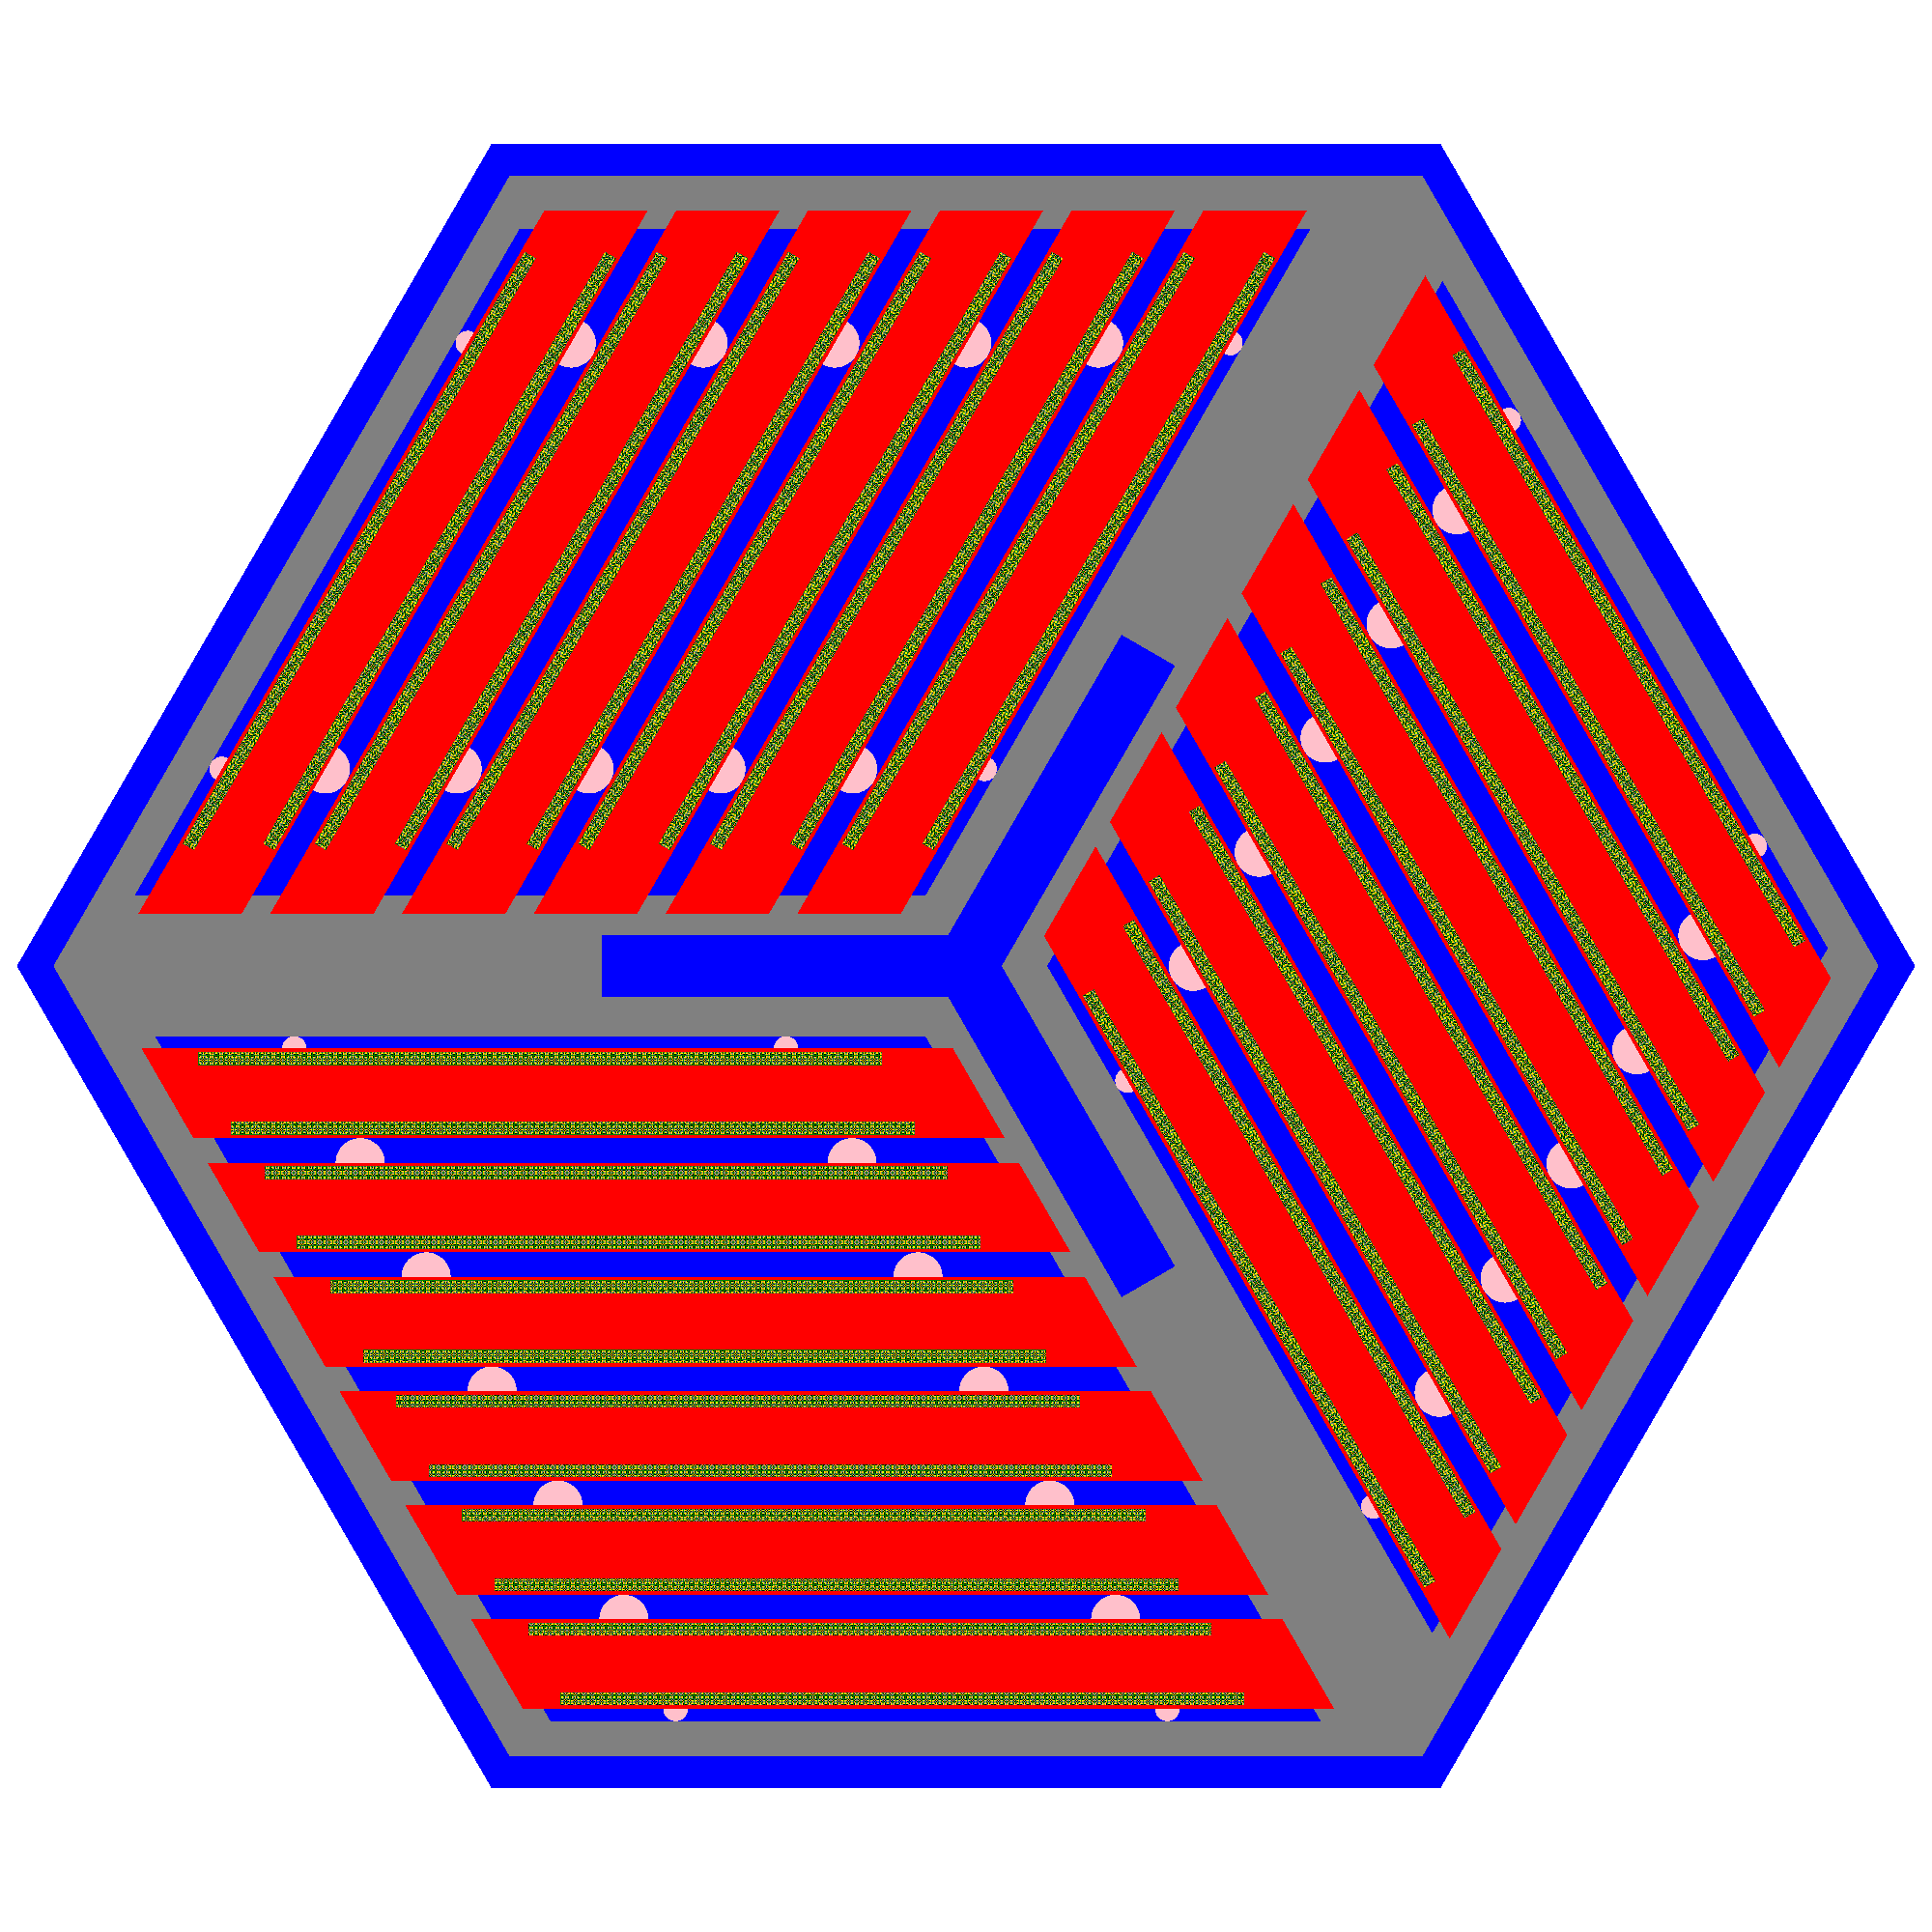
\includegraphics[width=0.5\linewidth]{ahtr-fuel-element.png} 
    \caption{FHR fuel element.}
    \label{fig:ahtr-fuel-element}
\end{figure}

The external channel wrapper and structural Y-shape as seen in Figure 
\ref{fig:y-shape} are made of C-C composite and have extra notches for the 
fuel plates to slide in. 
The gap between the fuel elements and fuel plates are filled with \gls{FLiBe}
coolant. 
At the center of the Y-shape structure is the Y-shaped control blade slot, 
which contains \gls{FLiBe} coolant when the control blade is not in the slot
\cite{varma_ahtr_2012,ramey_monte_2018,noauthor_fluoride_nodate}.

\begin{figure}[]
    \centering
    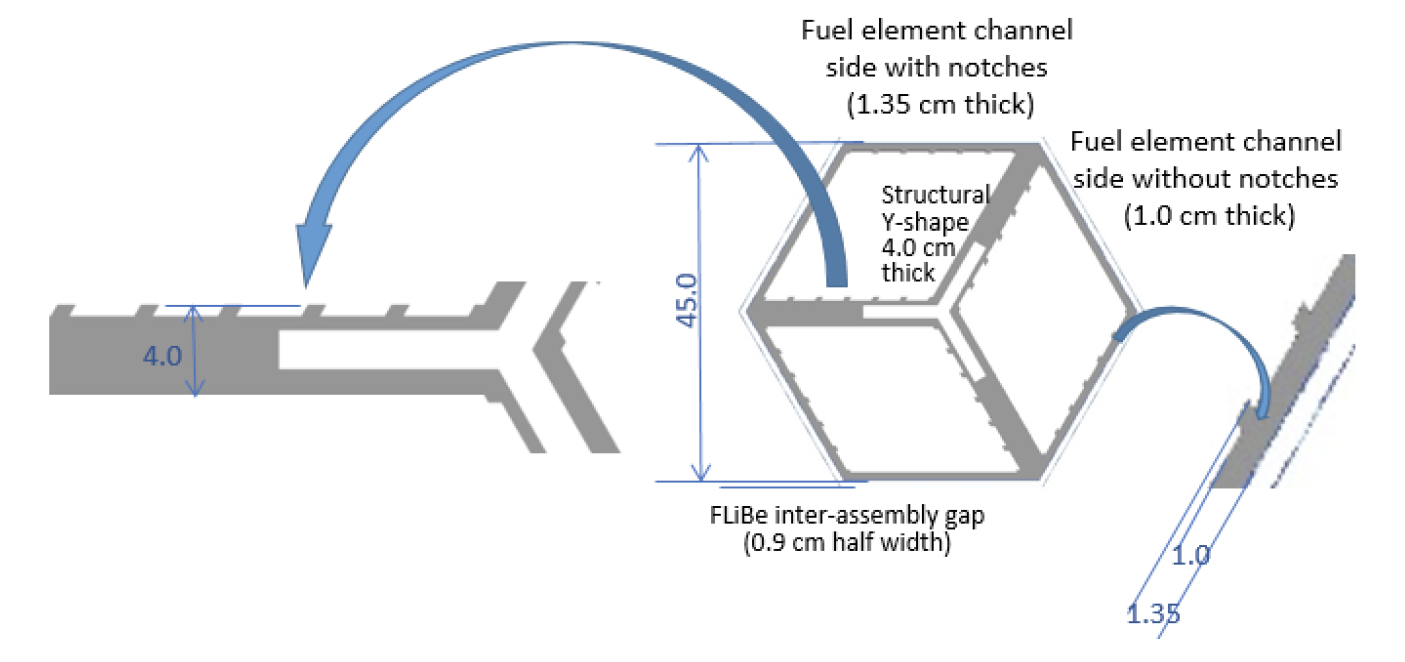
\includegraphics[width=0.8\linewidth]{y-shape.png} 
    \caption{FHR fuel element's structural components \cite{noauthor_fluoride_nodate}.}
    \label{fig:y-shape}
\end{figure}

Each fuel plank is made of an isostatically pressed carbon with fuel stripes 
on each outer side of the plank as seen in Figure \ref{fig:ahtr-fuel-plank}. 
The fuel stripes are prismatic regions composed of a graphite matrix filled with 
a cubic lattice of \gls{TRISO} particles. 
The lattice is 210 \gls{TRISO} particles wide in x-direction, 4 particles deep in 
the y-direction, and 5936 particles tall in the z-direction. 
Each \gls{TRISO} particle has 5 layers: Oxycarbide fuel kernel, porous carbon 
buffer, inner pyrolytic carbon, silicon carbide layer, and the outer pyrolitic 
carbon as seen in Figure \ref{fig:ahtr-triso}

\begin{figure}[]
    \centering
    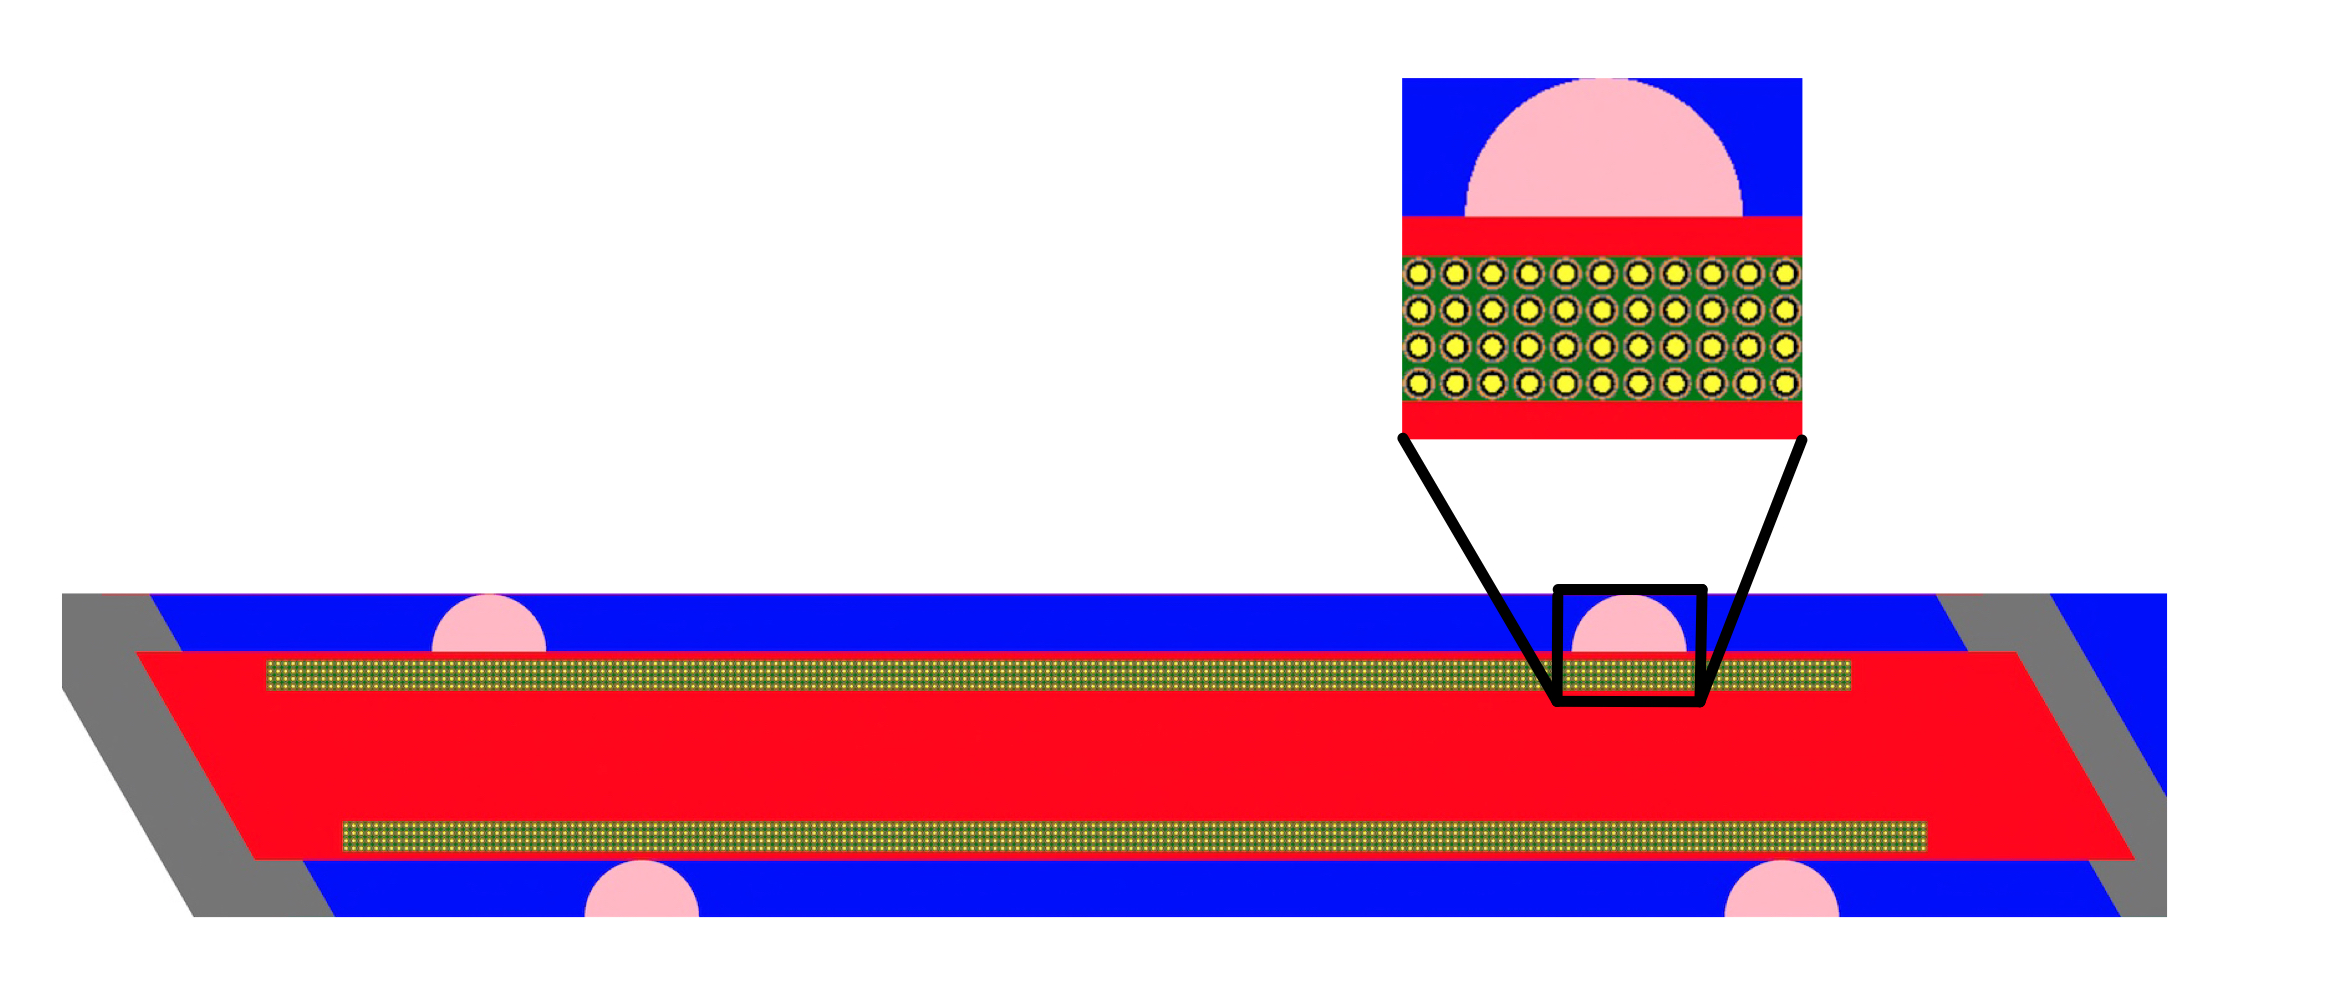
\includegraphics[width=0.8\linewidth]{ahtr-fuel-plank.png} 
    \caption{2D view of FHR fuel plank.}
    \label{fig:ahtr-fuel-plank}
\end{figure}

\begin{figure}[]
    \centering
    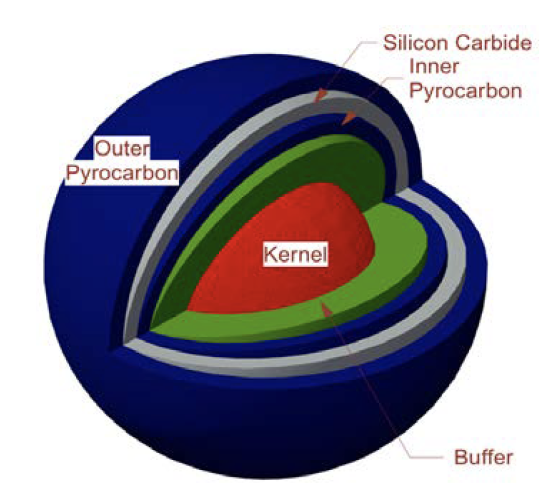
\includegraphics[width=0.4\linewidth]{ahtr-triso.png} 
    \caption{TRISO particle schematic \cite{noauthor_fluoride_nodate}.}
    \label{fig:ahtr-triso}
\end{figure}

\section{Results}